\section*{Lezione 18}
\addcontentsline{toc}{section}{Lezione 18}

\subsection*{Substitution-Permutation Network (SPN)}
\addcontentsline{toc}{subsection}{Substitution-Permutation Network (SPN)}
\textbf{Confusione e diffusione}: principi introdotti da Shannon, l'obiettivo è quello di rendere l'analisi statistica del testo cifrato $c$ molto difficile. L'idea è quella che le proprietà statistiche di $c$ devono essere indipendenti (al limite della fattibilità) dal valore di $k$. Definisce quindi il concetto di \textbf{diffusione} (spalmare), secondo cui la struttura statistica di $c$ è distribuita lungo tutta la lunghezza della chiave, ogni simbolo di $m$ ha effetto su \textit{più simboli} di $c$, e i simboli di $c$ sono determinati da più simboli di $m$. Per ottenere questo risultato si effettua una permutazione, seguita dall'applicazione di una funzione non lineare.\\
La \textbf{confusione}(ingarbugliare): la modifica di $m$ e/o di $k$ deve avere un output "imprevedibile", che non hanno relazioni statistiche fra di loro. Per ottenere questo effetto si usa una complessa sostituzione.\\
\textbf{Effetto valanga}: un piccolo cambiamento su $m$ o $k$ (anche un singolo bit), produce una modifica significativa (anche metà dei bit) di $c$.

Per mettere tutto insieme si usa una rete di permutazione e sostituzione (SPN, Substitution-Permutation Network).

\begin{figure}[h]
	\centering
	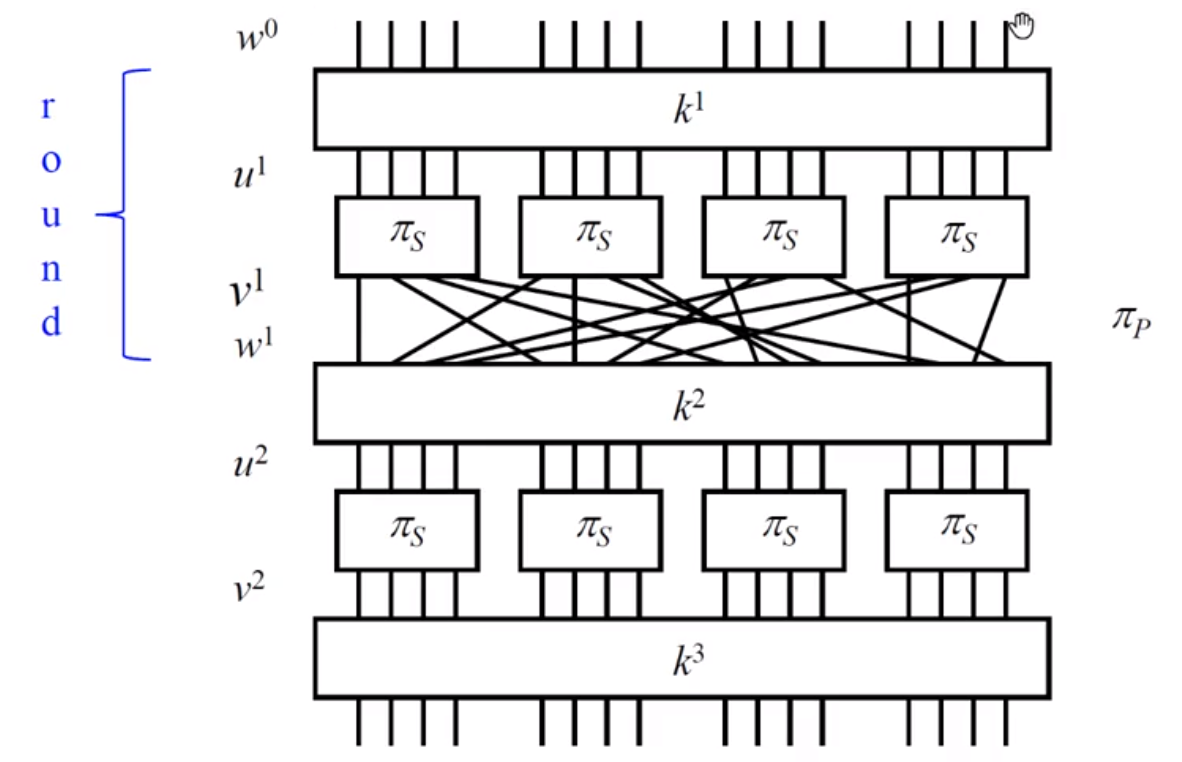
\includegraphics[width=0.85\linewidth]{immagini/img43}
\end{figure}
...

\subsection*{Struttura di Feistel}

\begin{figure}[h]
	\centering
	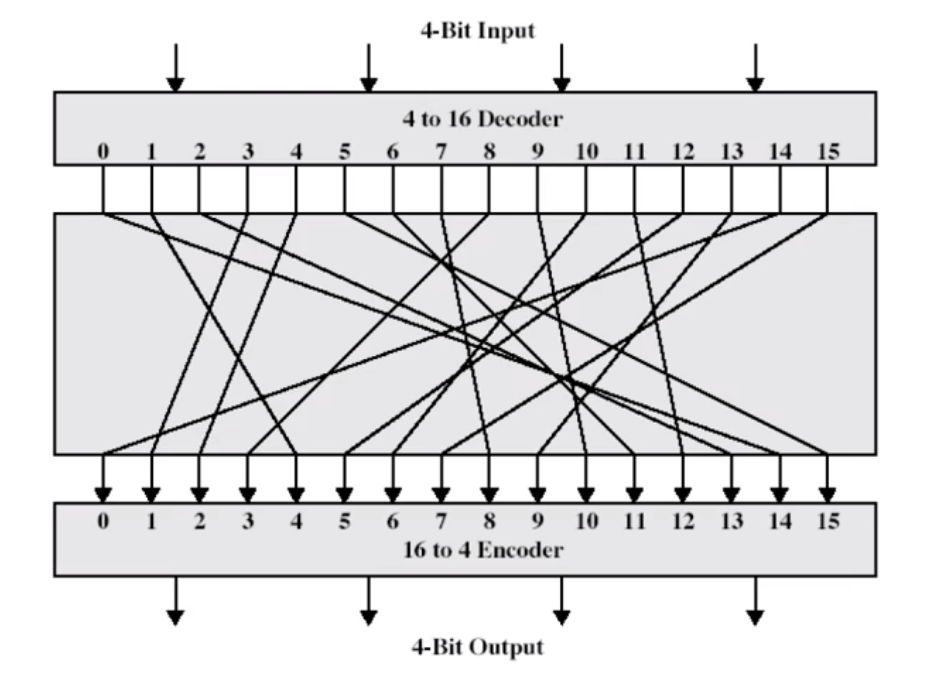
\includegraphics[width=0.85\linewidth]{immagini/img44}
\end{figure}
Le operazioni di cifratura devono essere invertibili. Dato un blocco di $n$ bit, la cifratura può essere espressa come la composizione di:
\begin{itemize}
	\item Un decoder da $n$ a $2^n$
	\item Una sostituzione monoalfabetica di $2^n$ simboli
	\item Un encoder da $2^n$ a $n$
\end{itemize}
Il problema è che dovrei salvare le $2^n$ sostutizioni, che diventano un casino.
L'idea è quella di implementare queste operazione usando dei moduli piccoli e facili da implementare (product ciphers)

La struttura di Feistel è un caso particolare di SPN:
\begin{itemize}
	\item input: testo in chiaro $m$ e una chiave $k$
	\item dalla chiave $k$ si generano le chiavi derivate $k^1, k^2, ..., k^n$
	\item $m$ è diviso in due metà: $L_0$ e $R_0$
	\item $L_0,R_0$ sono trasformate in $L_1,R_1, L_2,R_2, ..., L_n,R_n$ in $n$ round
\end{itemize}
In ogni round:
\begin{itemize}
	\item input: $L_{i-1}, R_{i-1}, k^i$, output: $L_i,R_i$
	\item sostituzione: una round function $F$ è applicata a $R_{i-1}$ e $k^i$, poi si effettua lo xor fra il risultato e $L_{i-1}$
	\item permutazione: $L_{i-1}$ e $R_{i-1}$ sono scambiati: $L_i=R_i$, $R_i=L_{i-1} \oplus F(R_{i-1}, k^i)$.
\end{itemize}
Dopo tutti i round, si elimina l'ultima permutazione (che non aggiunge sicurezza ma velocizza la decifratura).

\begin{figure}[h]
	\centering
	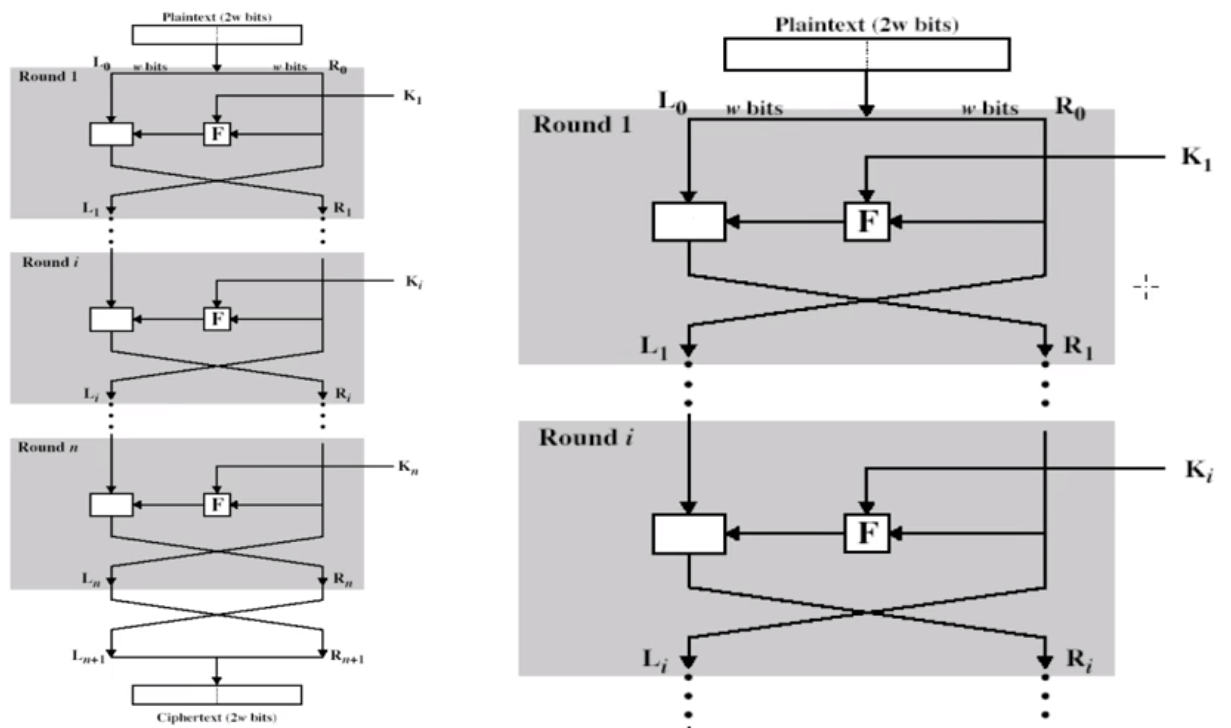
\includegraphics[width=\linewidth]{immagini/img45}
\end{figure}

Più le chiavi e i blocchi sono grandi, più il sistema è sicuro (ma lento).\\
Più round ci sono (effetto valanga) più il sistema è sicuro (ma lento).\\
Più è complicata $F$ più il sistema è sicuro (ma lento).\\
Più la generazione delle chiavi derivate è complicata, più il sistema è sicuro (ma lento).

Una qualità della Struttura di Feistel è che è completamente simmetrico, quindi la cifratura e la decifratura sono processi uguali (cambia solo l'ordine di utilizzo delle chiavi).


\subsubsection*{Crittoanalisi lineare} 
(faccio veloce, non chiede orale)\\
Coppersmith nel '94 dice che 
\begin{center}
	\textit{Nessun bit di output di una S-box dev'essere troppo vicino a una funzione lineare dei bit di input. In particolare, se selezioniamo un qualsiasi bit di output in qualunque sottoinsieme dei sei bit di input, la porzione di input per cui questo bit di output è uguale allo xor di questi bit di input non dovrebbe essere vicina a 0 o a 1, ma piuttosto vicina a $\frac12$}
\end{center}

\subsubsection*{Timing attack}
In base al tempo con cui vengono effettuate certe operazioni, traggo delle conclusioni. Sul DES si può trovare il numero di 1 nella chiave.

\subsubsection*{Design delle S-box}
\addcontentsline{toc}{subsubsection}{Design delle S-box}
Le S-box del DES sono fatte a mano, facendo dei tentativi e cercando di capire se i tentativi funzionano o no (molto lungo, nessuno fa più così).
Oppure le faccio a caso e scelgo solo quelle che soddisfano dei test statistici.
Oppure le S-box di AES sono definite sfruttando criteri matematici, in particolare la wide-trail strategy: posso provare a sostituire con funzioni lineari, ma queste coinvolgerebbero così tanti bit che renderebbero infattibile l'attacco di crittoanalisi lineare.


\subsubsection*{Cifrario a flusso}
\addcontentsline{toc}{subsubsection}{Cifrario a flusso}
Un cifrario che cifra un bit o un byte alla volta, cambiando continuamente la chiave, usando un keystream. La chiave segreta $k$ è usata come \textit{seed} per un PRNG (Pseudo-Random Number Generator) che produce le chiavi derivate, ognuna di un bit o byte.
Successivamente ogni bit o byte $m$ è calcolato facendo lo xor con l'output del generatore pseudo-casuale.

Il cifrario a flusso è sicuro se il generatore di numeri pseudo-casuali è buono (xor con bit casuali produce bit casuali).
Essi sono anche più veloci (usano meno codice), però non possiamo riutilizzare le chiavi (altrimenti creo delle relazioni lineari fra la porzione di chiave utilizzata e i testi in chiaro-cifrati, quindi il flusso di chiavi dev'essere aperiodico (al limite del fattibile)).
La sicurezza quindi è basata fortemente sull'algoritmo con cui genero un keystream robusto. Il seme (chiave) dev'essere abbastanza lungo (almento 128 bits) per evitare attacchi di forza bruta.

Per costruire le chiavi derivate uso LFSR (Linear Feedback Shift Registers), registro di scorrimento con feedback lineare. 

\begin{figure}[h]
	\centering
	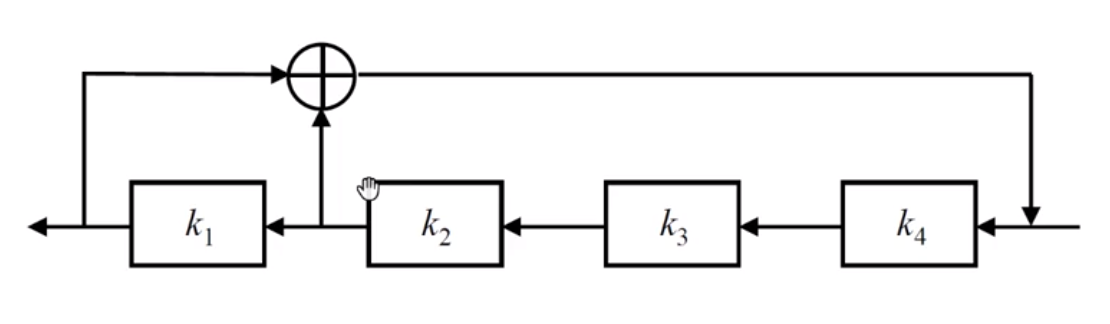
\includegraphics[width=0.85\linewidth]{immagini/img46}
\end{figure}

Ad ogni colpo di clock il contenuto di $k_4$ va a $k_3$, quello di $k_3$ a $k_2$ e così via

bla bla

Produce un output però che è generato usando equazioni lineari. Se Eve conoscesse $2m$ chiavi derivate, chiamate $z_1,z_2,...z_{2m}$ allora può scrviere un sistema di equazioni per ricavare la chiave. Quindi non usarli mai da soli.

\subsection*{RC4}
\addcontentsline{toc}{subsection}{RC4}

Cifrario a flusso più famoso, usato in SSL/TLS che sono gli standard per la comunicazione attraverso browser web, servizi di e-commerce ecc.

Come funziona?
\begin{itemize}
	\item Cifra un byte per volta
	\item Usa una permutazione casuale
	\item Usa un vettore di stato $S$ di 256 bit
	\item Usa una chiave $k$ che va da 1 a 256 byte per inizializzare $S$; dopodichè $k$ non è più utilizzata
	\item Il periodo del keystream arriva a $10^{100}$
	\item Richiede solo 8-16 operazioni macchina
\end{itemize}

Vediamo ora passo passo:
\begin{enumerate}
	\item Inizializzazione di $S$:\\
	Si mettono in $S$ tutti i numeri da 0 a 255, uso un vettore temporaneo $T$ in cui salvo la chiave $k$ tante volte quanto necessario per riempirlo (se la chiave è 256 byte allora apposto).
	\medskip
	
	\begin{algorithmic}
		\For {$i = 0$ to 255}
		\State $S[i] = i$
		\State $T[i] = k[i mod $ keylen $]$
		\EndFor
	\end{algorithmic}

	Successivamente ogni elemento di $S$ viene scambiato con un altro elemento, la cui posizione è determinatata da $S$ e $T$
	
	\medskip
	
	\begin{algorithmic}
		\State $j=0$
		\For {$i = 0$ to 255}
		\State $j = (j + S[i] + T[i])$ mod 256
		\State \textbf{swap}($S[i]], S[j]$)
		\EndFor
	\end{algorithmic}

	\item Generazione del keystream:\\
	Si parte da $S[0]$ e si arriva a $S[255]$, poi di nuovo da $S[0]$ e così via. Ad ongi interazione l'elemento $S[i]$ è cambiato con un altro elemento $S[j]$, dove il valore $j$ dipende da $S[i]$. La somma $S[i]+S[j]$ (mod 256) da la posizione dell'elemento $z$
	
	\medskip
	
	\begin{algorithmic}
		\State $j=0$
		\State $i=0$
		\While {\texttt{true}}
		\State {$i = (i+1)$ mod 256}
		\State {$j = (j+S[i])$ mod 256}
		\State \textbf{swap}($S[i], S[j]$)
		\State $t = (S[i] + S[j]) mod 256$
		\State $z=S[t]$
		\EndWhile
	\end{algorithmic}

\item Cifratura e decifratura:\\
La cifratura è lo xor fra il testo e $z$: $c_i = m_i \cdot z$, la decifratura il contrario: $m_i = c_i \cdot z$.
Non si conoscono attacchi che rompano l'algoritmo (a parte l'implementazione WEP)

\end{enumerate}

\subsection*{La sicurezza di Shannon}
Shannon si chiede, esiste un crittosistema sicuro incondizionatamente? Anche AES-256, se ha un computer della madonna ce la fa dopo un po'. Basta avere una coppia testo + testo cifrato e provare tutte le $2^{256}$.

Chiamiamo $X$ una variabile casuale che assume valori in $PT$ (spazio dei testi in chiaro), $Y$ una variabile casuale che assume valori in $CT$ (spazio dei testi cifrati).
Alice sceglie $x \in PT$, lo cifra, ottiene $y \in CT$ e lo manda a Bob.\\
Per semplicità mettiamo che Alice scelga $x$ con una probabilità normale uniforme.
Eve conosce solo $P[X=x]$. Se però intercetta il messaggio cifrato $y$, conosce $P[X=x]$ e $P[X=x|Y=y]$ (probabilità all'indietro).

Per Shannon il crittosistema è sicuro se Eve non impara nulla dopo aver conosciuto la probabilità all'indietro:
\begin{equation*}
\forall x \in X, y \in Y
\end{equation*}
\begin{equation*}
Prob[X=x] = Prob[X=x|Y=y]
\end{equation*}
che equivale a:
\begin{equation*}
H(X) = H(X|Y)
\end{equation*}
che sarebbe $I(X;Y) = 0$ (la mutua informazione del sistema vale 0), quindi $X$ e $Y$ sono indipendenti, quindi Eve non ottiene alcuna informazione da $y$.\\
Questo vuol dire che il canale sarebbe completamente rumoroso. Un crittosistema di questo tipo esiste ed è il \textbf{One Time Pad}.
Esso ha una chiave lunga tanto quanto il testo e dev'essere utilizzata una sola volta. Si cifra e decifra facendo lo xor fra la chiave e il testo. Una proprietà di OTP è $\forall y, \forall k, \exists x : E_k(x) = y$, in altre parole la $y$ può essere generata da ogni $x$ utilizzando una chiave adatta. Quindi la $y$ non ci da alcun informazione. Basta che la chiave sia di un bit più corta per far sì che non sia più incondizionatamente sicuro, visto che $Prob[X=x|Y=y]=\frac1{2^{n-1}} \neq Prob[X=x]$.

Ovviamente ha dei contro:
\begin{itemize}
	\item Bisogna produrre grandi quantità di chiavi casuali (ogni chiave poi sarà buttata)
	\item Bisogna distribuire e proteggere le chiavi
	\item Difficile da gestire
\end{itemize}





